\documentclass[11pt]{article}
\usepackage[textwidth=18.0cm, textheight=23.0cm, top=2.0cm]{geometry}
\usepackage{pst-all}
\usepackage{amssymb}
\usepackage{tikz}
\usepackage{underscore}\begin{document}
\pagestyle{empty}


ClassName: \underline{\textbf{Class_08.2bp-17}}
\par
BinSize: \underline{\textbf{100 × 100}}
\par
ReduceSize: \underline{\textbf{100 × 100}}
\par
TypeNum: \underline{\textbf{40}}
\par
Num: \underline{\textbf{40}}
\par
OutS: \underline{\textbf{110000}}
\par
InS: \underline{\textbf{91811}}
\par
Rate: \underline{\textbf{0.835}}
\par
UB: \underline{\textbf{11}}
\par
LB0: \underline{\textbf{11}}
\par
LB: \underline{\textbf{11}}
\par
LBWithCut: \underline{\textbf{11}}
\par
NodeCut: \underline{\textbf{0}}
\par
ExtendedNodeCnt: \underline{\textbf{1}}
\par
GenNodeCnt: \underline{\textbf{1}}
\par
PrimalNode: \underline{\textbf{0}}
\par
ColumnCount: \underline{\textbf{11}}
\par
TotalCutCount: \underline{\textbf{0}}
\par
RootCutCount: \underline{\textbf{0}}
\par
LPSolverCnt: \underline{\textbf{1}}
\par
PricingSolverCnt: \underline{\textbf{0}}
\par
BranchAndBoundNum: \underline{\textbf{1}}
\par
isOpt: \underline{\textbf{true}}
\par
TimeOnInitSolution: \underline{\textbf{0.060 s}}
\par
TimeOnPrimal: \underline{\textbf{0.000 s}}
\par
TimeOnPricing: \underline{\textbf{0.000 s}}
\par
TimeOnRmp: \underline{\textbf{0.063 s}}
\par
TotalTime: \underline{\textbf{0.185 s}}
\par
\newpage


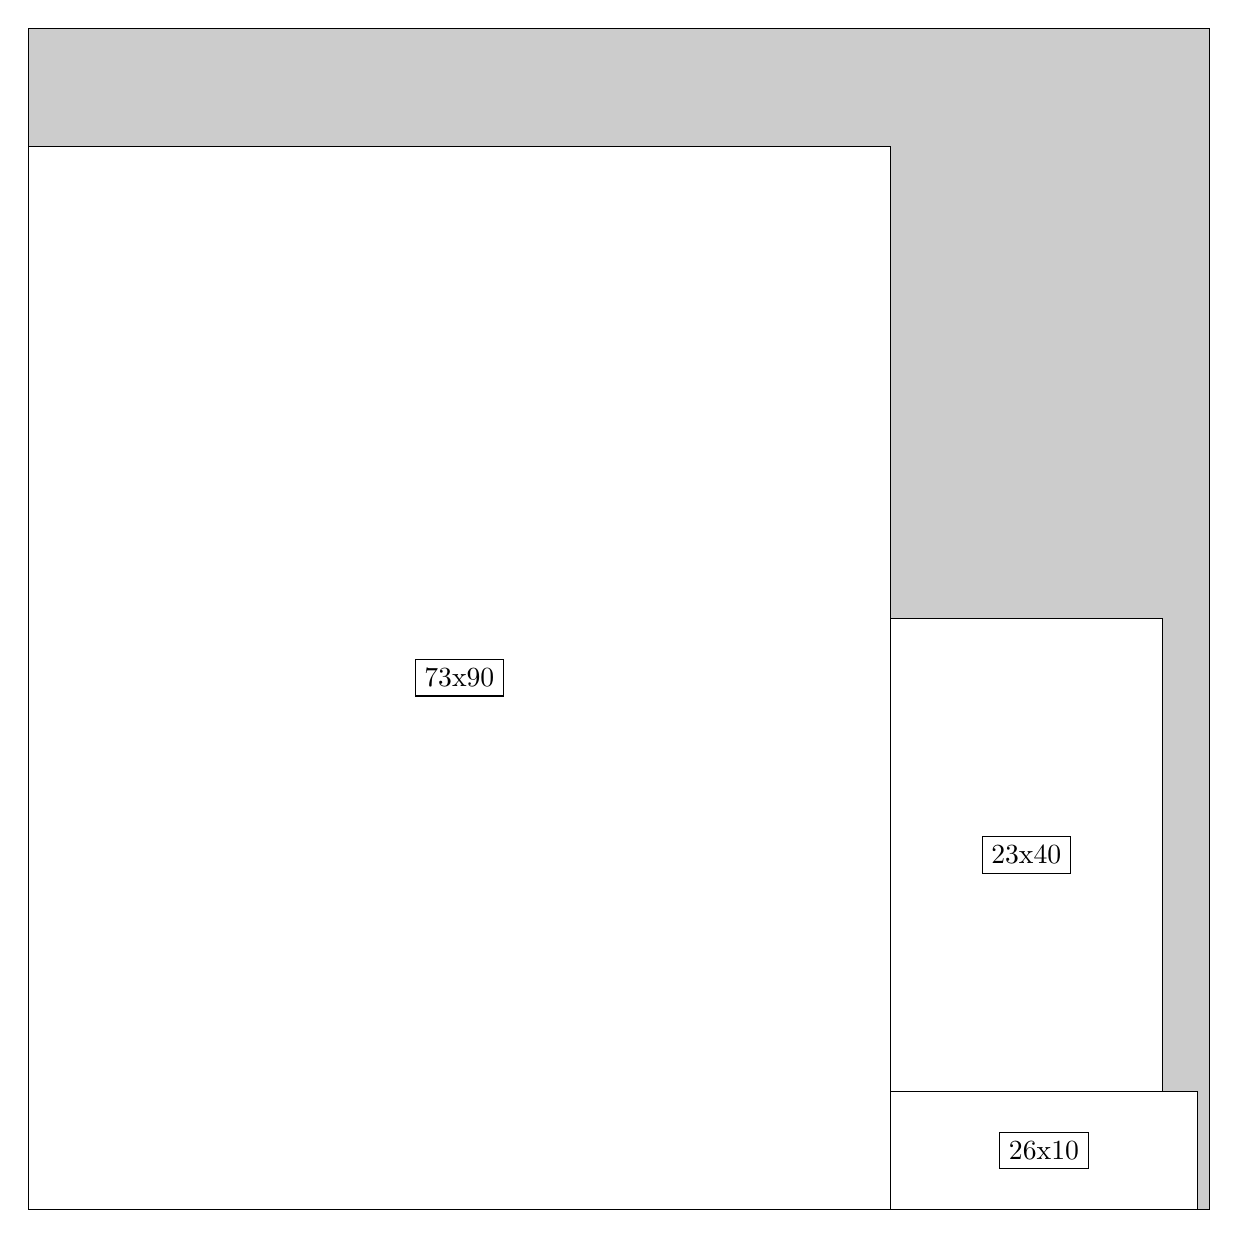
\begin{tikzpicture}[shorten >=1pt,scale=1.0,every node/.style={scale=1.0},->]
\tikzstyle{vertex}=[circle,fill=black!25,minimum size=14pt,inner sep=0pt]
\filldraw[fill=gray!40!white, draw=black] (0,0) rectangle (15.0,15.0);
\foreach \name/\x/\y/\w/\h in {73x90/0.0/0.0/10.95/13.5,23x40/10.95/1.5/3.4499999999999997/6.0,26x10/10.95/0.0/3.9/1.5}
\filldraw[fill=white!40!white, draw=black] (\x,\y) rectangle node[draw] (\name) {\name} ++(\w,\h);
\end{tikzpicture}


w =73 , h =90 , x =0 , y =0 , v =6570
\par
w =23 , h =40 , x =73 , y =10 , v =920
\par
w =26 , h =10 , x =73 , y =0 , v =260
\par
\newpage


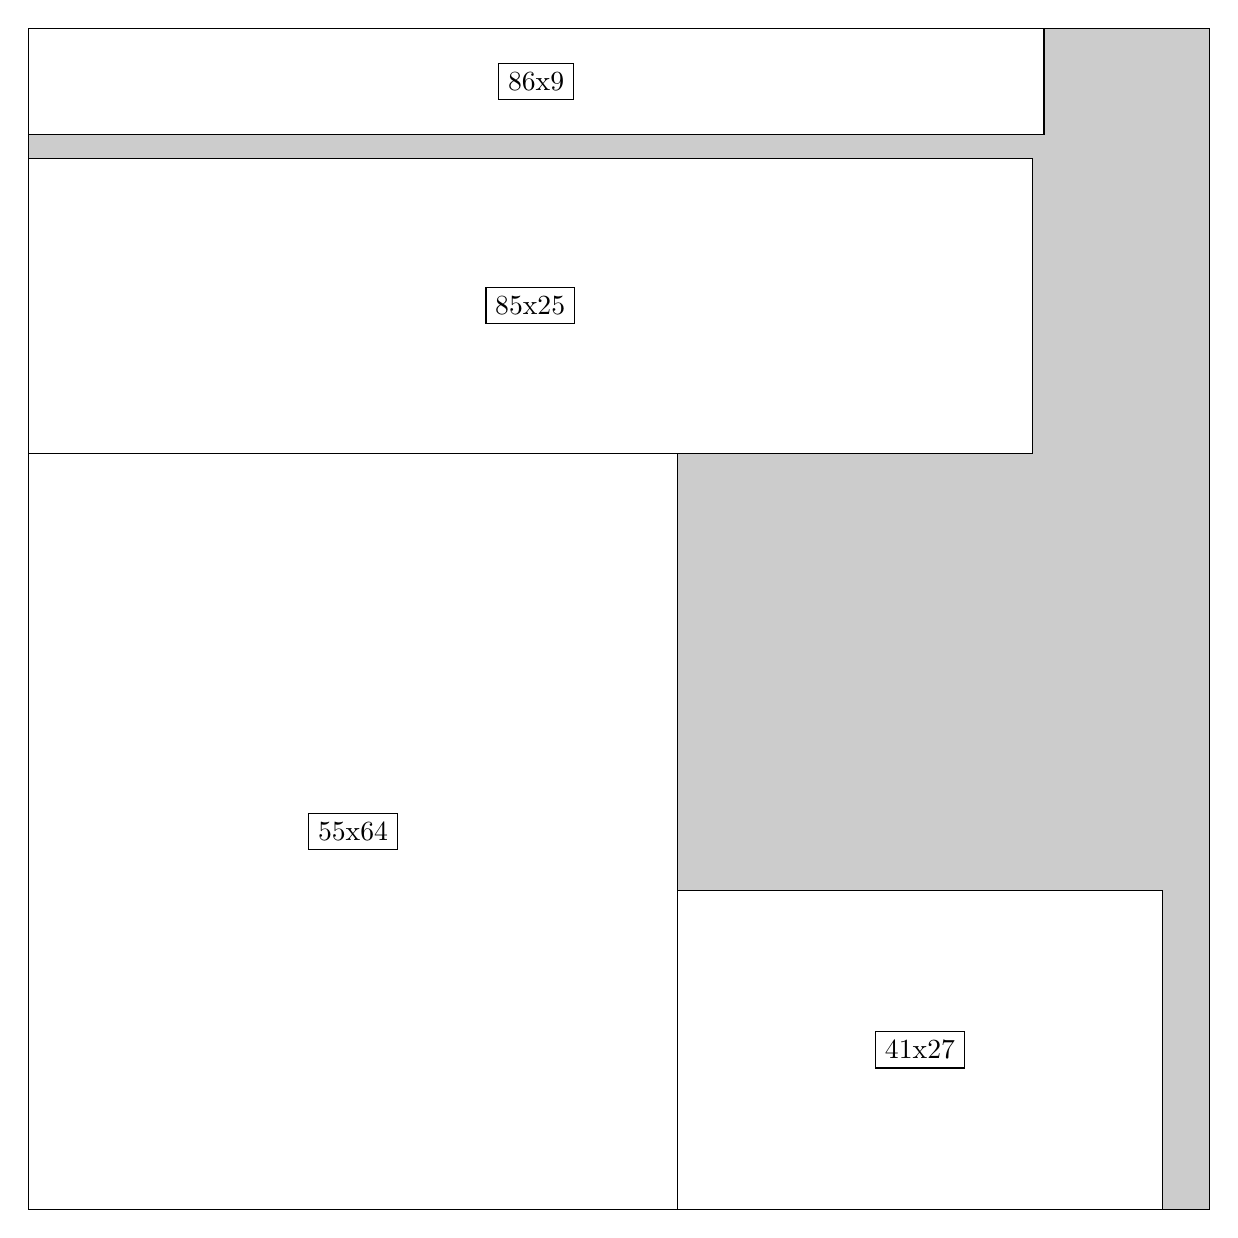
\begin{tikzpicture}[shorten >=1pt,scale=1.0,every node/.style={scale=1.0},->]
\tikzstyle{vertex}=[circle,fill=black!25,minimum size=14pt,inner sep=0pt]
\filldraw[fill=gray!40!white, draw=black] (0,0) rectangle (15.0,15.0);
\foreach \name/\x/\y/\w/\h in {55x64/0.0/0.0/8.25/9.6,85x25/0.0/9.6/12.75/3.75,41x27/8.25/0.0/6.1499999999999995/4.05,86x9/0.0/13.65/12.9/1.3499999999999999}
\filldraw[fill=white!40!white, draw=black] (\x,\y) rectangle node[draw] (\name) {\name} ++(\w,\h);
\end{tikzpicture}


w =55 , h =64 , x =0 , y =0 , v =3520
\par
w =85 , h =25 , x =0 , y =64 , v =2125
\par
w =41 , h =27 , x =55 , y =0 , v =1107
\par
w =86 , h =9 , x =0 , y =91 , v =774
\par
\newpage


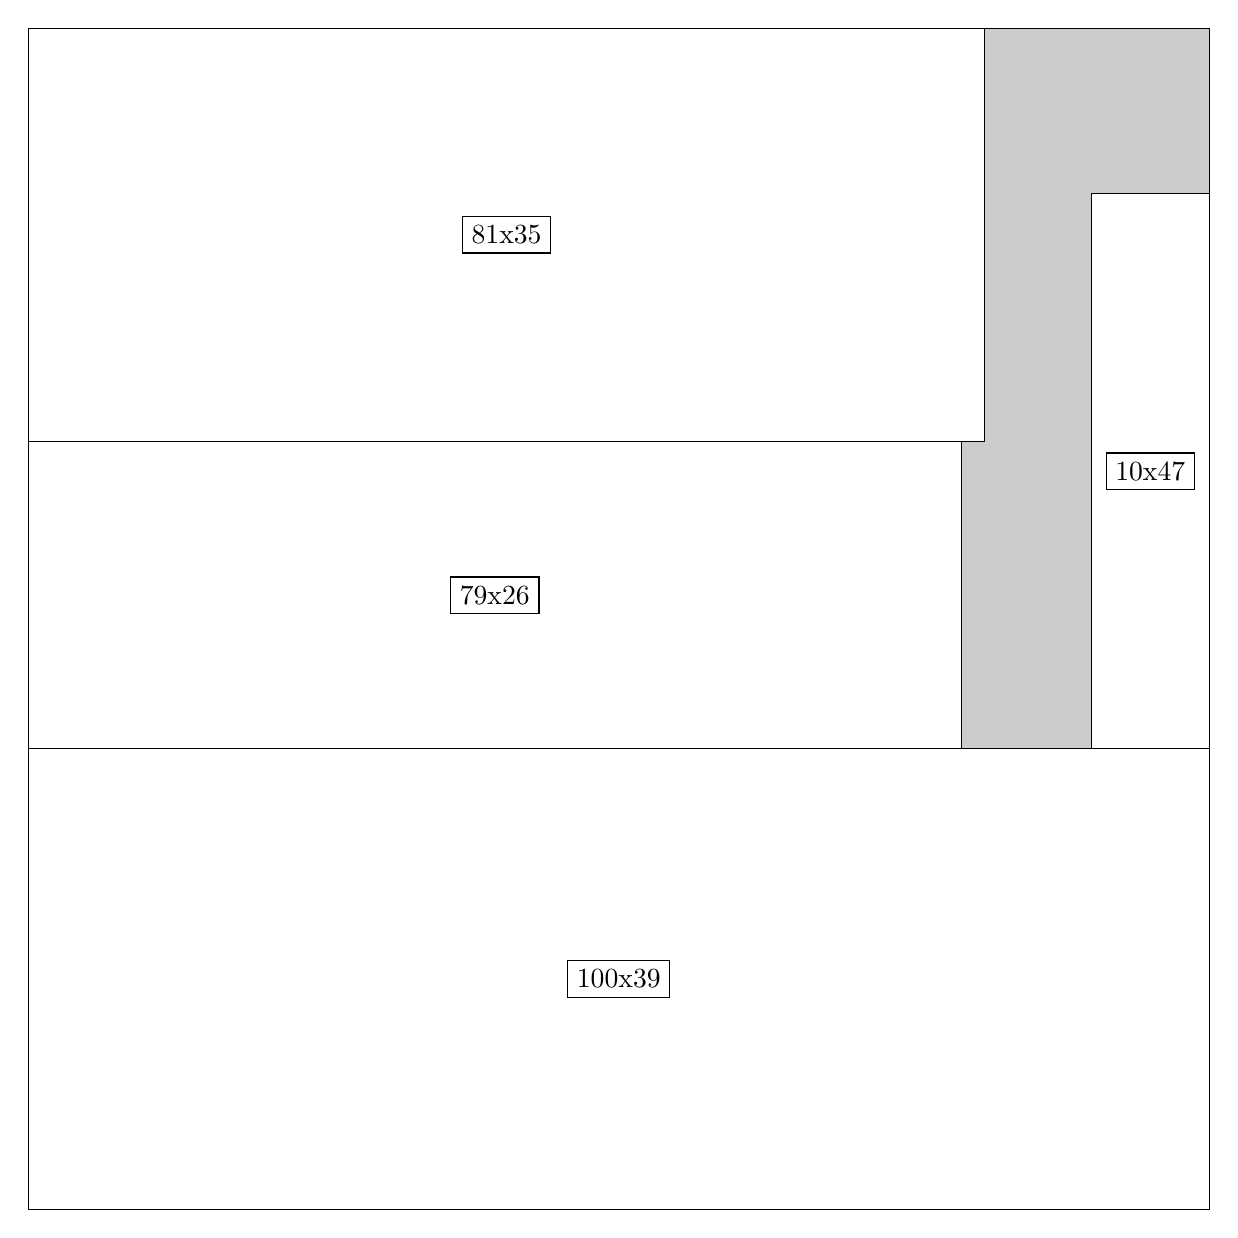
\begin{tikzpicture}[shorten >=1pt,scale=1.0,every node/.style={scale=1.0},->]
\tikzstyle{vertex}=[circle,fill=black!25,minimum size=14pt,inner sep=0pt]
\filldraw[fill=gray!40!white, draw=black] (0,0) rectangle (15.0,15.0);
\foreach \name/\x/\y/\w/\h in {79x26/0.0/5.85/11.85/3.9,100x39/0.0/0.0/15.0/5.85,81x35/0.0/9.75/12.15/5.25,10x47/13.5/5.85/1.5/7.05}
\filldraw[fill=white!40!white, draw=black] (\x,\y) rectangle node[draw] (\name) {\name} ++(\w,\h);
\end{tikzpicture}


w =79 , h =26 , x =0 , y =39 , v =2054
\par
w =100 , h =39 , x =0 , y =0 , v =3900
\par
w =81 , h =35 , x =0 , y =65 , v =2835
\par
w =10 , h =47 , x =90 , y =39 , v =470
\par
\newpage


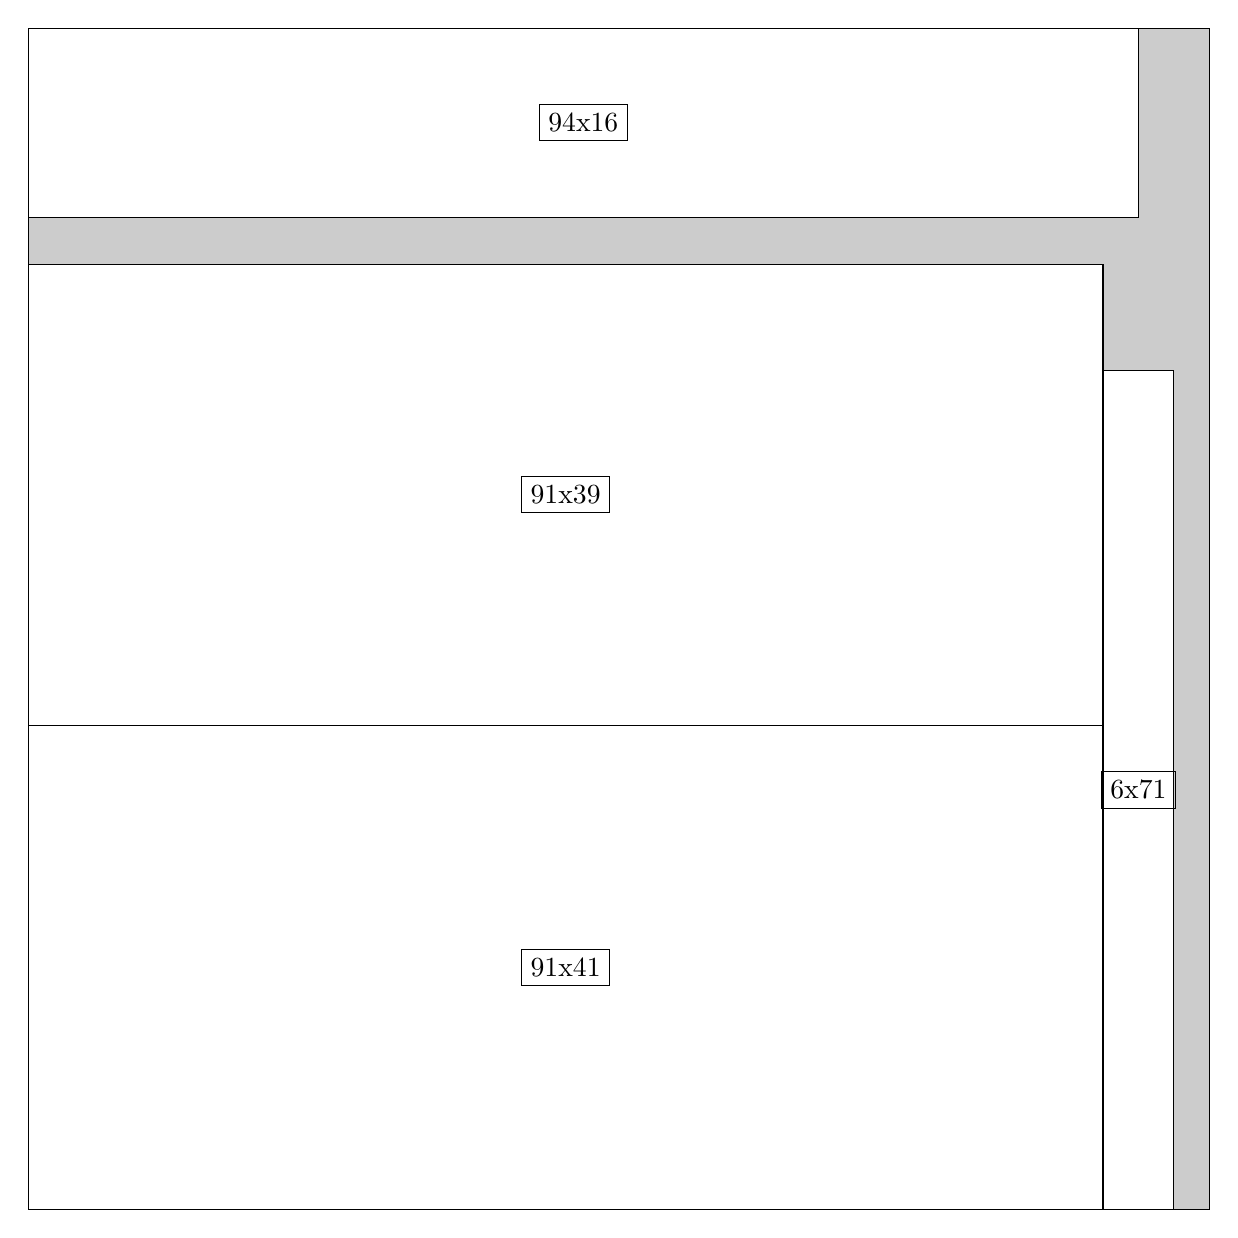
\begin{tikzpicture}[shorten >=1pt,scale=1.0,every node/.style={scale=1.0},->]
\tikzstyle{vertex}=[circle,fill=black!25,minimum size=14pt,inner sep=0pt]
\filldraw[fill=gray!40!white, draw=black] (0,0) rectangle (15.0,15.0);
\foreach \name/\x/\y/\w/\h in {91x41/0.0/0.0/13.65/6.1499999999999995,91x39/0.0/6.1499999999999995/13.65/5.85,94x16/0.0/12.6/14.1/2.4,6x71/13.65/0.0/0.8999999999999999/10.65}
\filldraw[fill=white!40!white, draw=black] (\x,\y) rectangle node[draw] (\name) {\name} ++(\w,\h);
\end{tikzpicture}


w =91 , h =41 , x =0 , y =0 , v =3731
\par
w =91 , h =39 , x =0 , y =41 , v =3549
\par
w =94 , h =16 , x =0 , y =84 , v =1504
\par
w =6 , h =71 , x =91 , y =0 , v =426
\par
\newpage


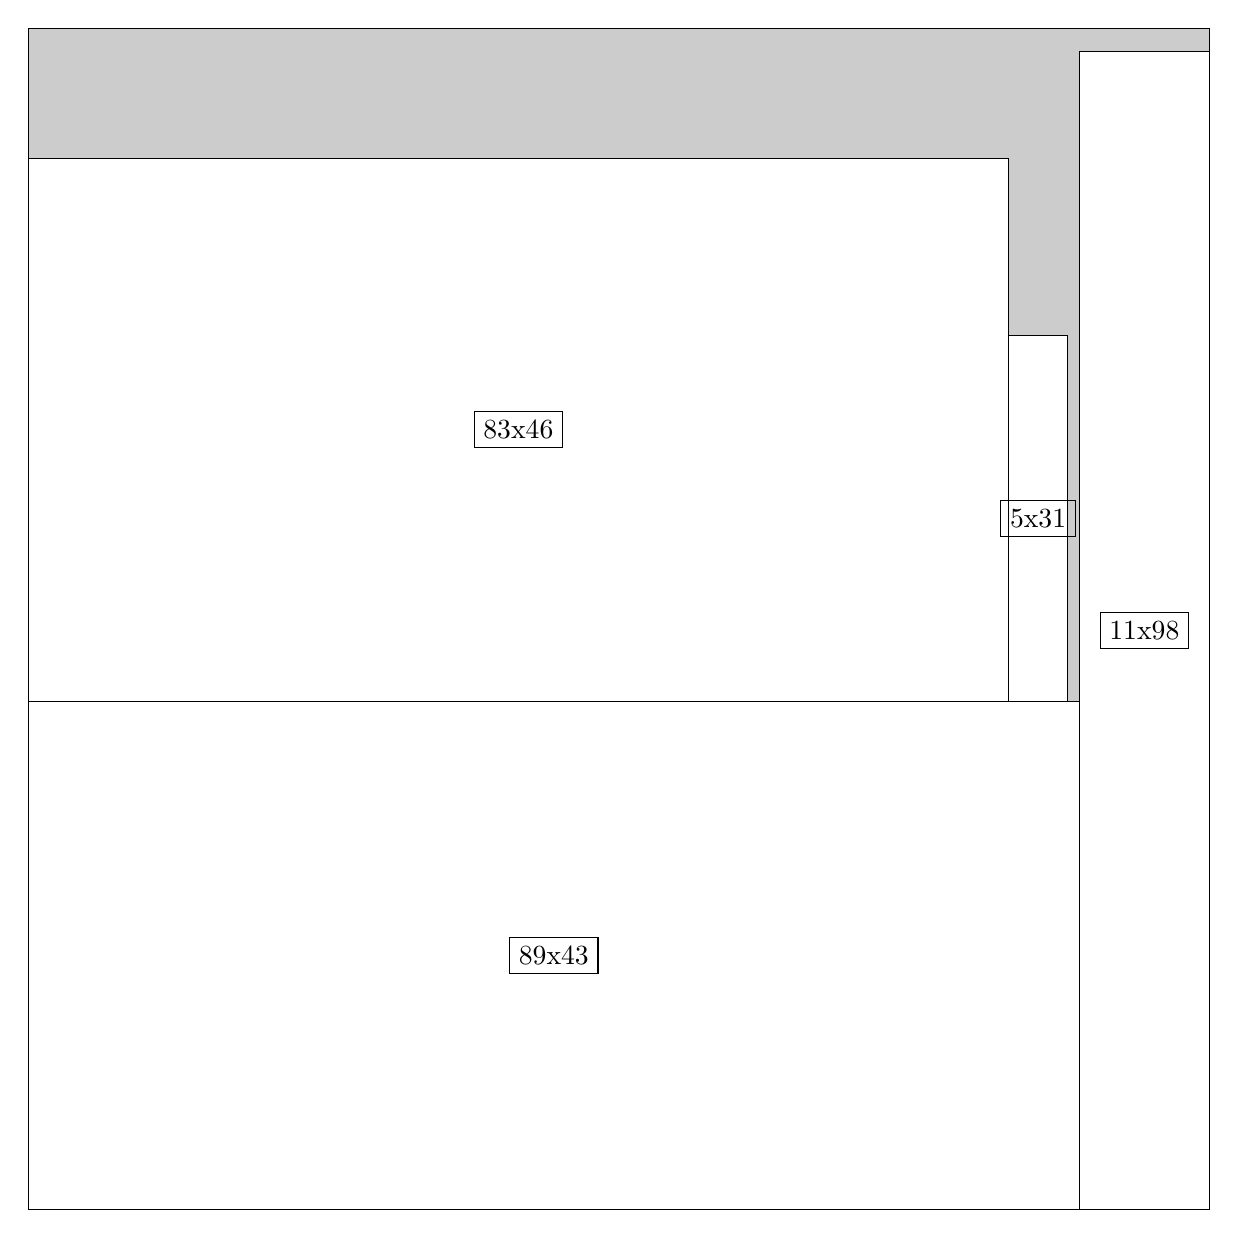
\begin{tikzpicture}[shorten >=1pt,scale=1.0,every node/.style={scale=1.0},->]
\tikzstyle{vertex}=[circle,fill=black!25,minimum size=14pt,inner sep=0pt]
\filldraw[fill=gray!40!white, draw=black] (0,0) rectangle (15.0,15.0);
\foreach \name/\x/\y/\w/\h in {89x43/0.0/0.0/13.35/6.45,83x46/0.0/6.45/12.45/6.8999999999999995,11x98/13.35/0.0/1.65/14.7,5x31/12.45/6.45/0.75/4.6499999999999995}
\filldraw[fill=white!40!white, draw=black] (\x,\y) rectangle node[draw] (\name) {\name} ++(\w,\h);
\end{tikzpicture}


w =89 , h =43 , x =0 , y =0 , v =3827
\par
w =83 , h =46 , x =0 , y =43 , v =3818
\par
w =11 , h =98 , x =89 , y =0 , v =1078
\par
w =5 , h =31 , x =83 , y =43 , v =155
\par
\newpage


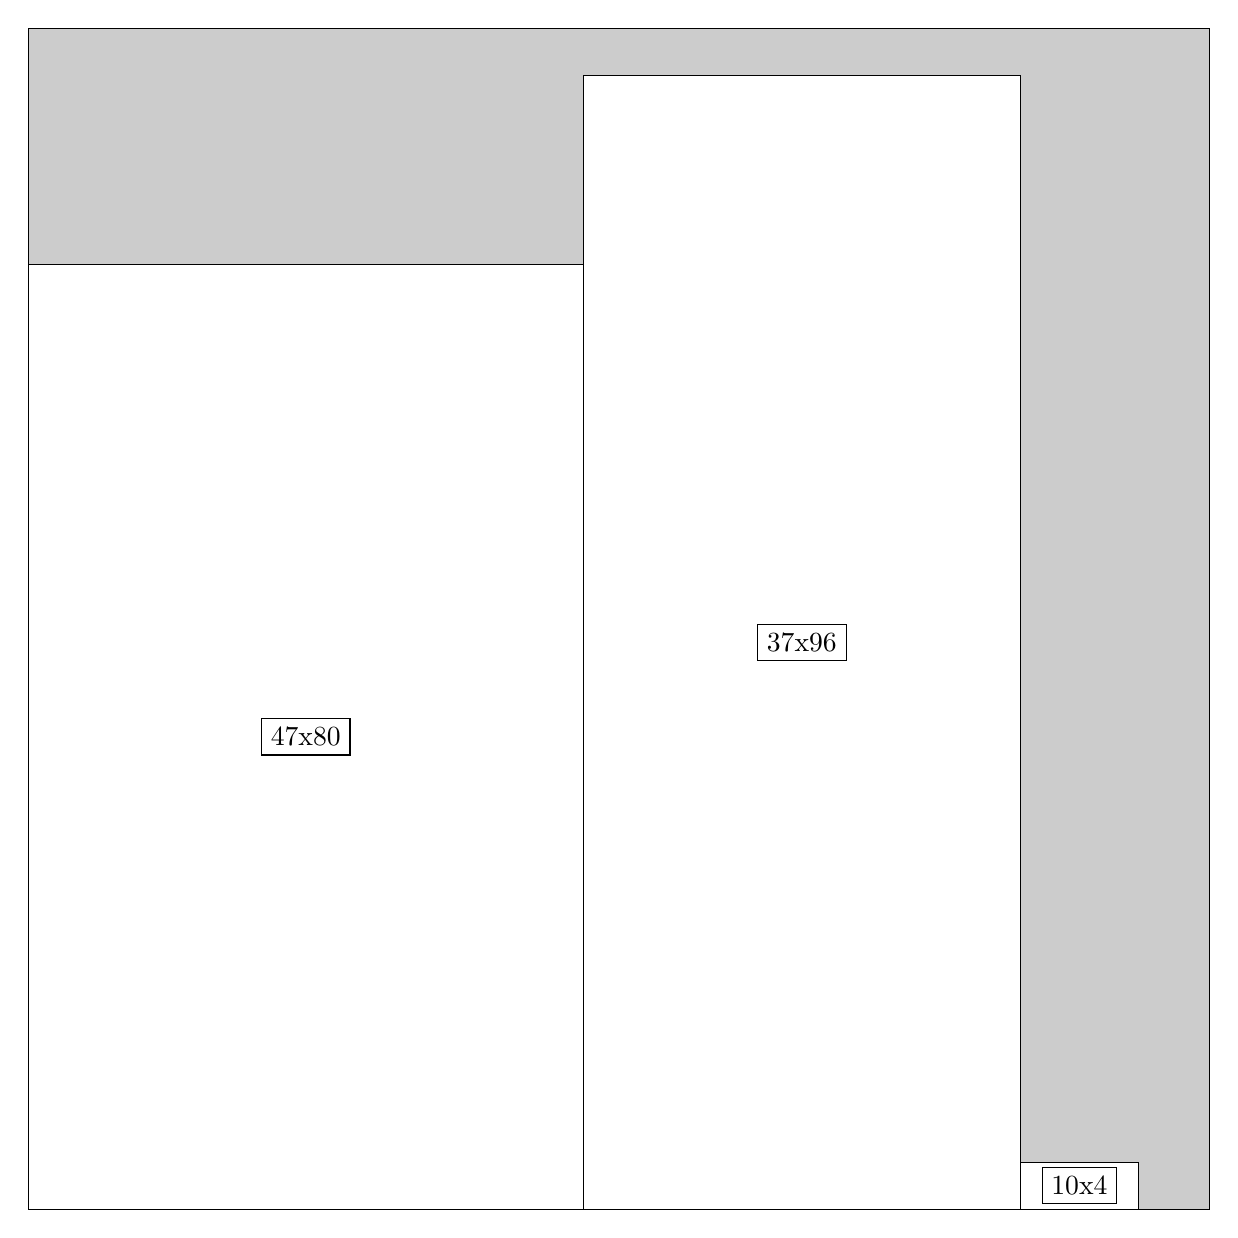
\begin{tikzpicture}[shorten >=1pt,scale=1.0,every node/.style={scale=1.0},->]
\tikzstyle{vertex}=[circle,fill=black!25,minimum size=14pt,inner sep=0pt]
\filldraw[fill=gray!40!white, draw=black] (0,0) rectangle (15.0,15.0);
\foreach \name/\x/\y/\w/\h in {47x80/0.0/0.0/7.05/12.0,37x96/7.05/0.0/5.55/14.399999999999999,10x4/12.6/0.0/1.5/0.6}
\filldraw[fill=white!40!white, draw=black] (\x,\y) rectangle node[draw] (\name) {\name} ++(\w,\h);
\end{tikzpicture}


w =47 , h =80 , x =0 , y =0 , v =3760
\par
w =37 , h =96 , x =47 , y =0 , v =3552
\par
w =10 , h =4 , x =84 , y =0 , v =40
\par
\newpage


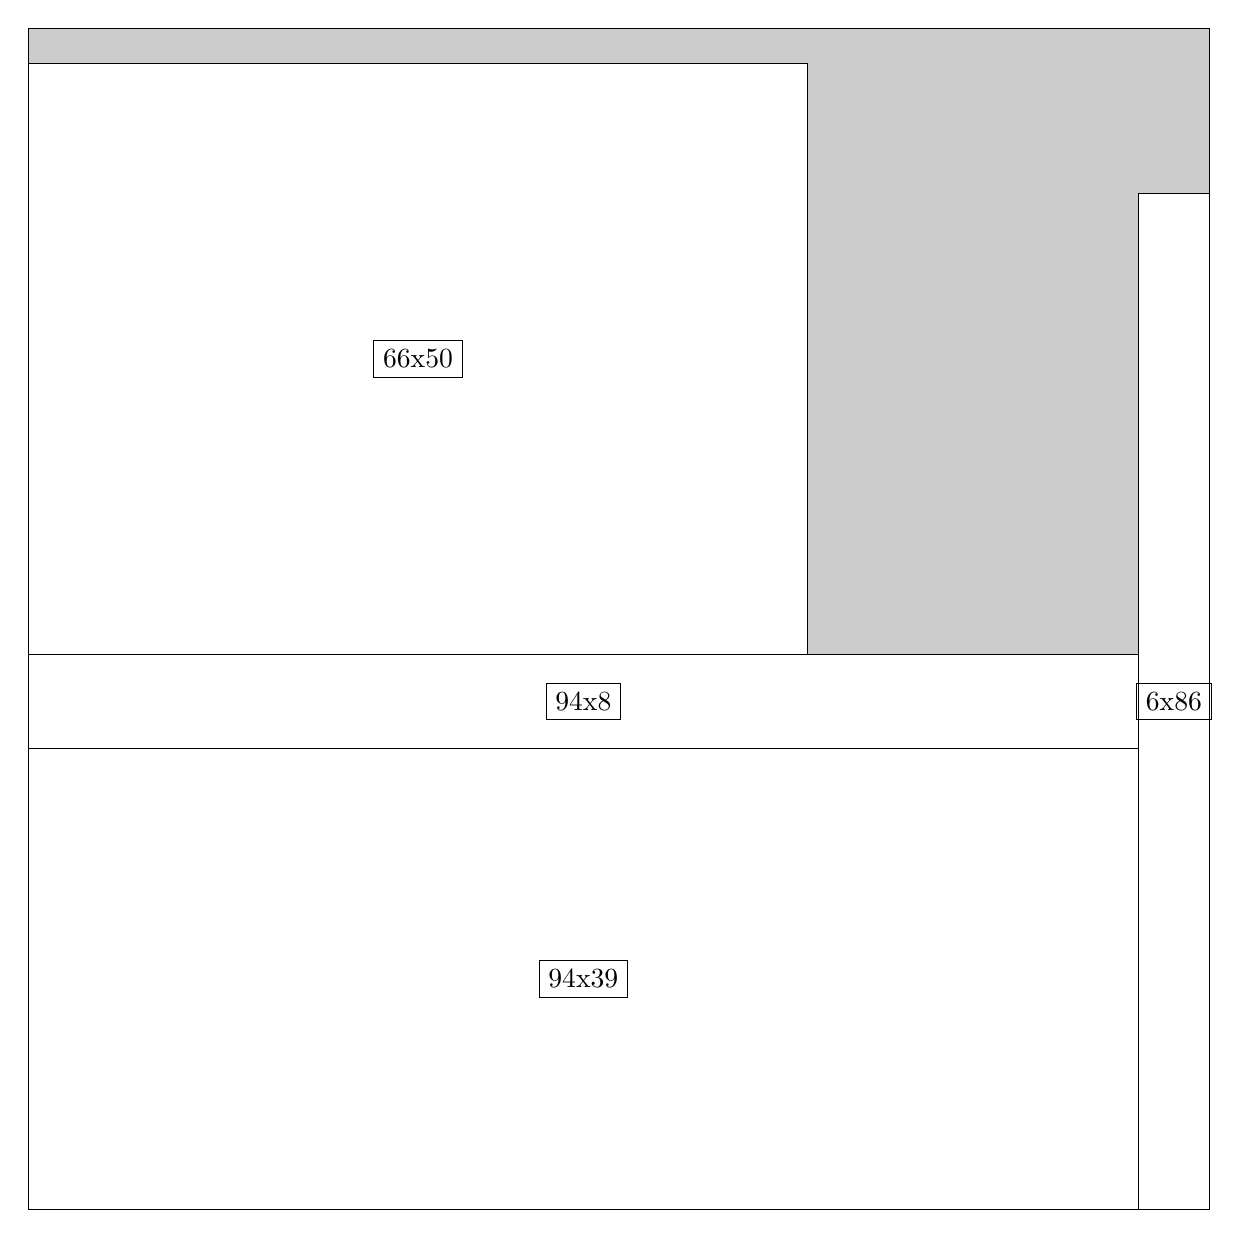
\begin{tikzpicture}[shorten >=1pt,scale=1.0,every node/.style={scale=1.0},->]
\tikzstyle{vertex}=[circle,fill=black!25,minimum size=14pt,inner sep=0pt]
\filldraw[fill=gray!40!white, draw=black] (0,0) rectangle (15.0,15.0);
\foreach \name/\x/\y/\w/\h in {94x39/0.0/0.0/14.1/5.85,66x50/0.0/7.05/9.9/7.5,94x8/0.0/5.85/14.1/1.2,6x86/14.1/0.0/0.8999999999999999/12.9}
\filldraw[fill=white!40!white, draw=black] (\x,\y) rectangle node[draw] (\name) {\name} ++(\w,\h);
\end{tikzpicture}


w =94 , h =39 , x =0 , y =0 , v =3666
\par
w =66 , h =50 , x =0 , y =47 , v =3300
\par
w =94 , h =8 , x =0 , y =39 , v =752
\par
w =6 , h =86 , x =94 , y =0 , v =516
\par
\newpage


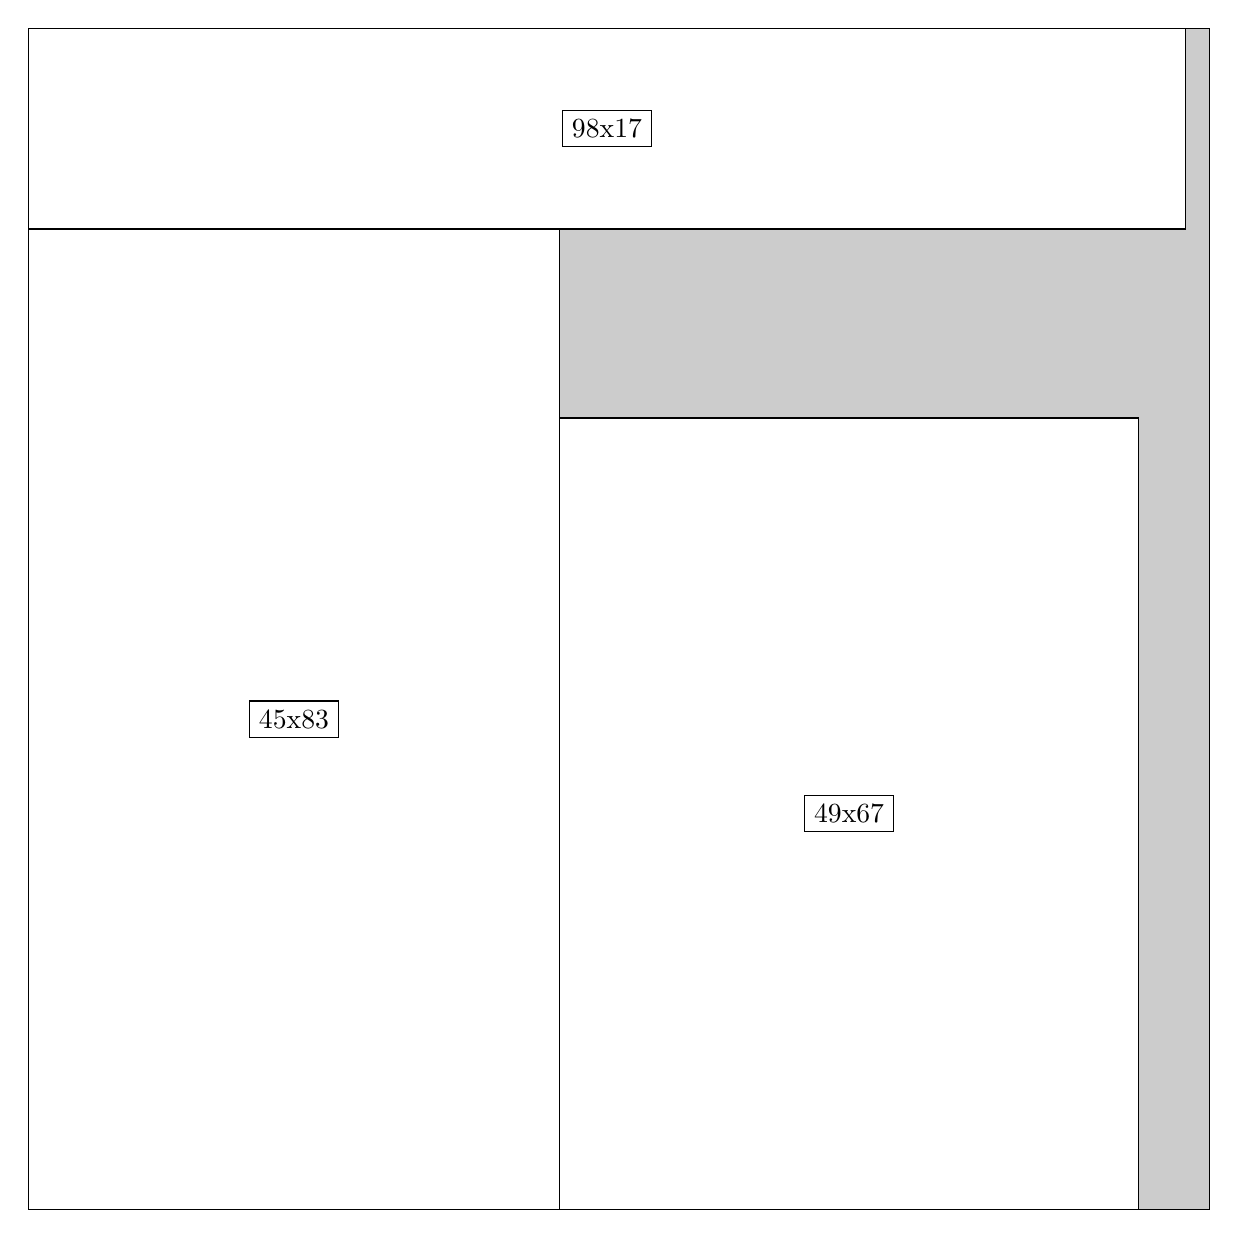
\begin{tikzpicture}[shorten >=1pt,scale=1.0,every node/.style={scale=1.0},->]
\tikzstyle{vertex}=[circle,fill=black!25,minimum size=14pt,inner sep=0pt]
\filldraw[fill=gray!40!white, draw=black] (0,0) rectangle (15.0,15.0);
\foreach \name/\x/\y/\w/\h in {45x83/0.0/0.0/6.75/12.45,49x67/6.75/0.0/7.35/10.049999999999999,98x17/0.0/12.45/14.7/2.55}
\filldraw[fill=white!40!white, draw=black] (\x,\y) rectangle node[draw] (\name) {\name} ++(\w,\h);
\end{tikzpicture}


w =45 , h =83 , x =0 , y =0 , v =3735
\par
w =49 , h =67 , x =45 , y =0 , v =3283
\par
w =98 , h =17 , x =0 , y =83 , v =1666
\par
\newpage


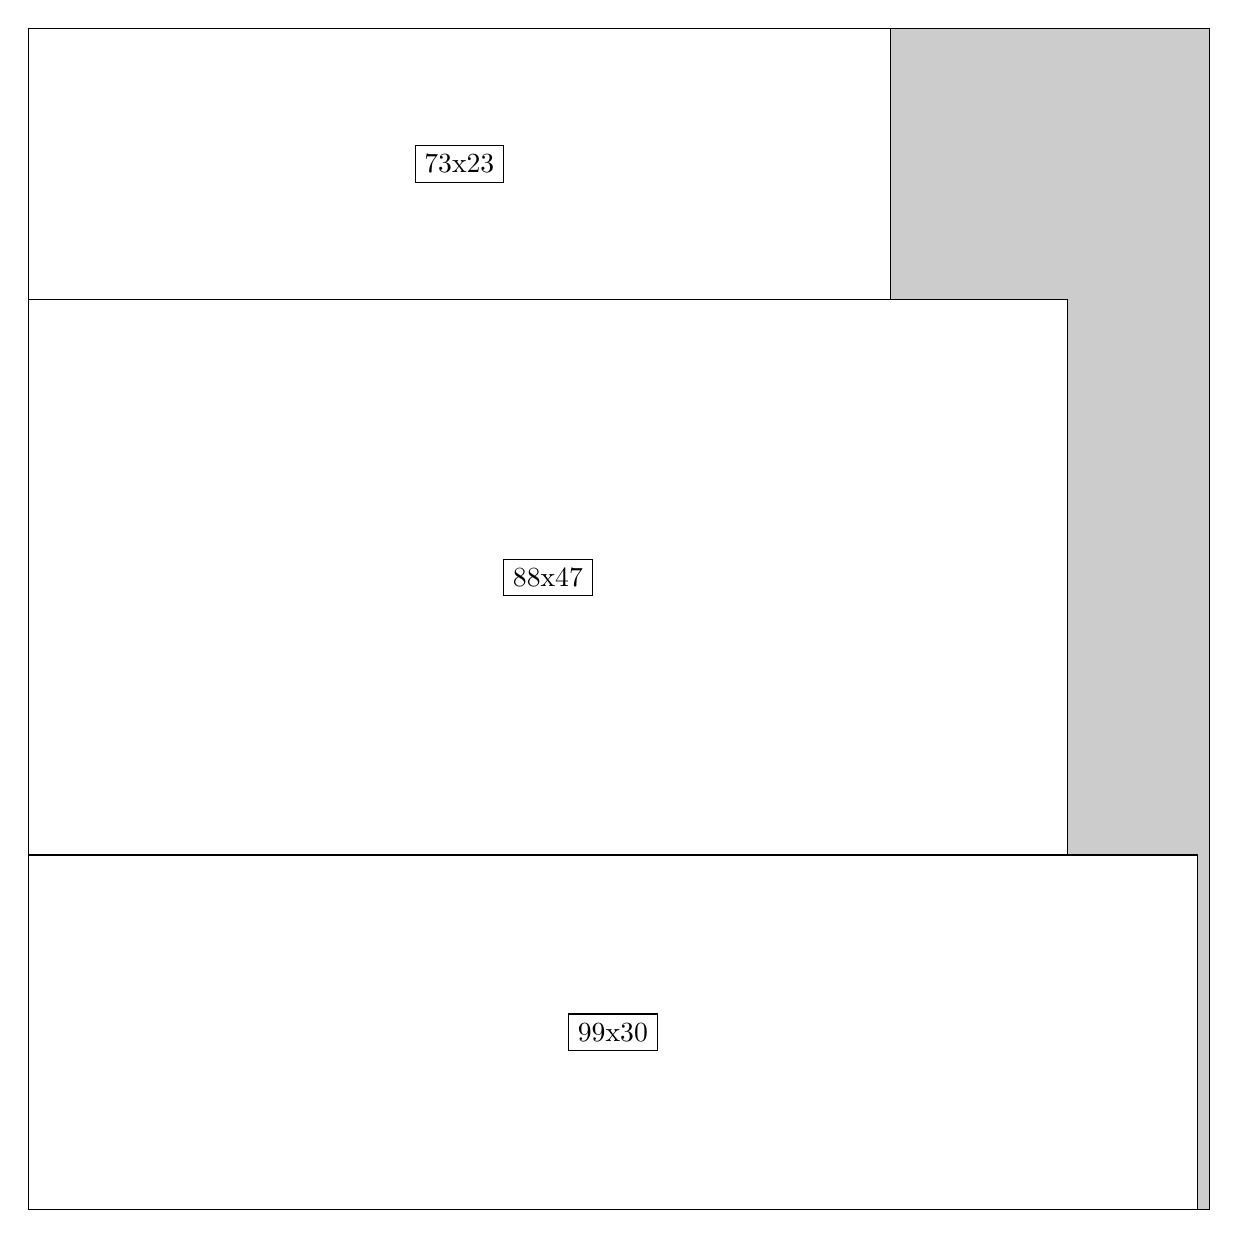
\begin{tikzpicture}[shorten >=1pt,scale=1.0,every node/.style={scale=1.0},->]
\tikzstyle{vertex}=[circle,fill=black!25,minimum size=14pt,inner sep=0pt]
\filldraw[fill=gray!40!white, draw=black] (0,0) rectangle (15.0,15.0);
\foreach \name/\x/\y/\w/\h in {99x30/0.0/0.0/14.85/4.5,88x47/0.0/4.5/13.2/7.05,73x23/0.0/11.549999999999999/10.95/3.4499999999999997}
\filldraw[fill=white!40!white, draw=black] (\x,\y) rectangle node[draw] (\name) {\name} ++(\w,\h);
\end{tikzpicture}


w =99 , h =30 , x =0 , y =0 , v =2970
\par
w =88 , h =47 , x =0 , y =30 , v =4136
\par
w =73 , h =23 , x =0 , y =77 , v =1679
\par
\newpage


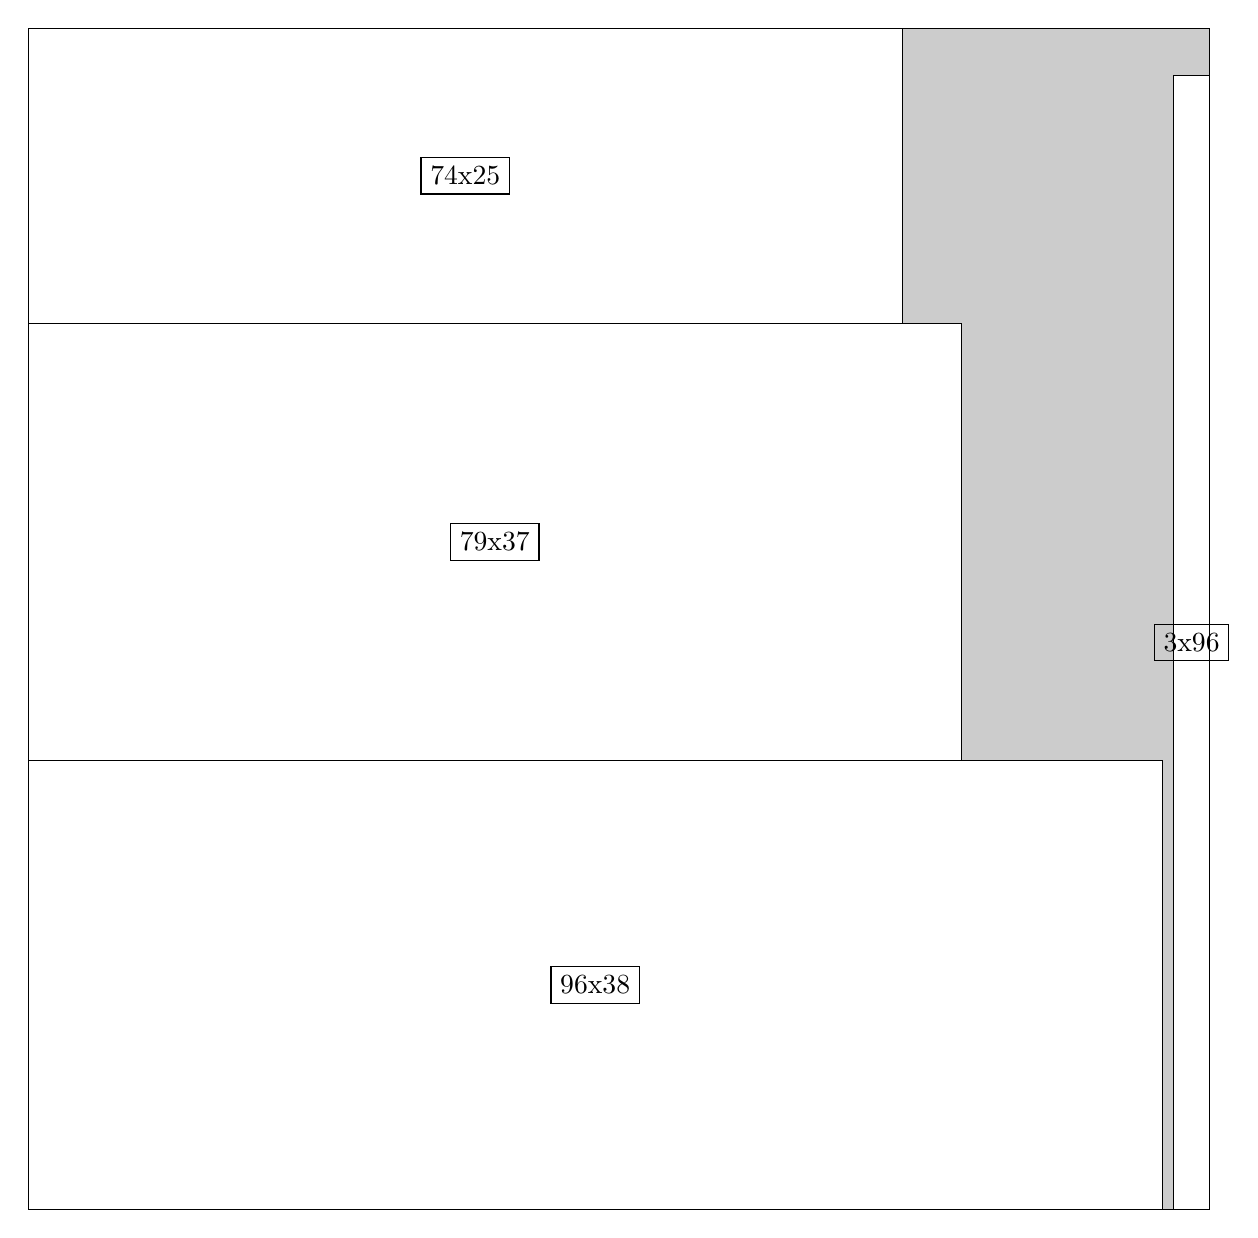
\begin{tikzpicture}[shorten >=1pt,scale=1.0,every node/.style={scale=1.0},->]
\tikzstyle{vertex}=[circle,fill=black!25,minimum size=14pt,inner sep=0pt]
\filldraw[fill=gray!40!white, draw=black] (0,0) rectangle (15.0,15.0);
\foreach \name/\x/\y/\w/\h in {96x38/0.0/0.0/14.399999999999999/5.7,79x37/0.0/5.7/11.85/5.55,74x25/0.0/11.25/11.1/3.75,3x96/14.549999999999999/0.0/0.44999999999999996/14.399999999999999}
\filldraw[fill=white!40!white, draw=black] (\x,\y) rectangle node[draw] (\name) {\name} ++(\w,\h);
\end{tikzpicture}


w =96 , h =38 , x =0 , y =0 , v =3648
\par
w =79 , h =37 , x =0 , y =38 , v =2923
\par
w =74 , h =25 , x =0 , y =75 , v =1850
\par
w =3 , h =96 , x =97 , y =0 , v =288
\par
\newpage


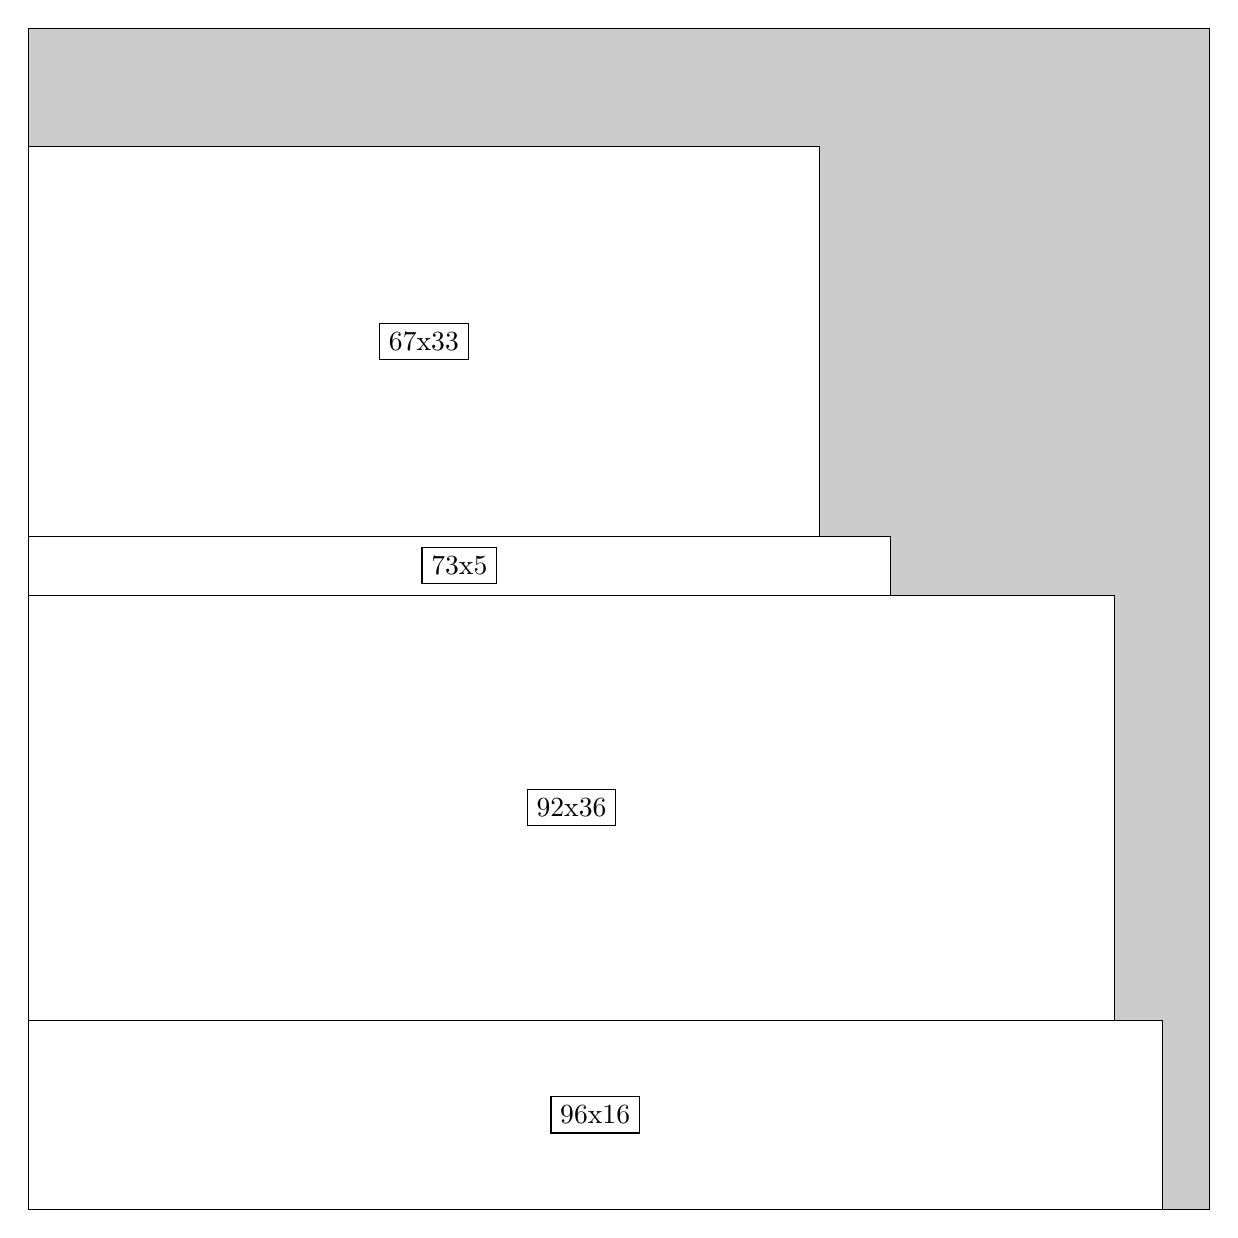
\begin{tikzpicture}[shorten >=1pt,scale=1.0,every node/.style={scale=1.0},->]
\tikzstyle{vertex}=[circle,fill=black!25,minimum size=14pt,inner sep=0pt]
\filldraw[fill=gray!40!white, draw=black] (0,0) rectangle (15.0,15.0);
\foreach \name/\x/\y/\w/\h in {92x36/0.0/2.4/13.799999999999999/5.3999999999999995,96x16/0.0/0.0/14.399999999999999/2.4,67x33/0.0/8.549999999999999/10.049999999999999/4.95,73x5/0.0/7.8/10.95/0.75}
\filldraw[fill=white!40!white, draw=black] (\x,\y) rectangle node[draw] (\name) {\name} ++(\w,\h);
\end{tikzpicture}


w =92 , h =36 , x =0 , y =16 , v =3312
\par
w =96 , h =16 , x =0 , y =0 , v =1536
\par
w =67 , h =33 , x =0 , y =57 , v =2211
\par
w =73 , h =5 , x =0 , y =52 , v =365
\par
\newpage


\end{document}